https://en.wikipedia.org/wiki/Advanced_Format

\documentclass[xga]{xdvislides}
\usepackage[landscape]{geometry}
\usepackage{array}
\usepackage{graphics}
\usepackage{graphicx}
\usepackage{colordvi}
\usepackage{tabularx}
\usepackage{multirow}

\begin{document}
\setfontphv

%%% Headers and footers
\lhead{\slidetitle}				% default:\lhead{\slidetitle}
\chead{CS615 - Aspects of System Administration}% default:\chead{\relax}
\rhead{Slide \thepage}				% default:\rhead{\sectiontitle}
\lfoot{\Gray{Lecture 02: Filesystems, Disks, Storage}}% default:\lfoot{\slideauthor}
\cfoot{\relax}					% default:\cfoot{\relax}
\rfoot{\Gray{\today}}

\vspace*{\fill}
\begin{center}
	\Hugesize
		CS615 - Aspects of System Administration\\ [1em]
		Filesystems, Disks, Storage\\ [1em]
	\hspace*{5mm}\blueline\\ [1em]
	\Normalsize
		Department of Computer Science\\
		Stevens Institute of Technology\\
		Jan Schaumann\\
		\verb+jschauma@stevens.edu+ \\
		\verb+https://www.cs.stevens.edu/~jschauma/615A/+
\end{center}
\vspace*{\fill}
%\setcounter{page}{0}
%\clearpage

\subsection{Let's review HW1}
\vspace{.5in}
Start all assignments on {\tt
linux-lab.cs.stevens.edu}! \\
\vspace{.5in}
Submit plain text. \\
\vspace{.5in}
No resubmissions.

\subsection{Let's review HW1}
\vspace{.5in}

Running an instance:
\begin{verbatim}
$ aws ec2 run-instances --instance-type t1.micro \
        --key-name stevens --image-id ami-569ed93c
\end{verbatim}

\subsection{Let's review HW1}
\vspace{.5in}

Save yourself some typing:
\begin{verbatim}
$ alias instance='aws ec2 run-instances --key-name stevens --image-id'
$ instance ami-569ed93c --instance-type t1.micro
\end{verbatim}

\subsection{Let's review HW1}
\vspace{.5in}

Make it permanent:
\begin{verbatim}
$ echo "alias instance='aws ec2 run-instances --key-name stevens --image-id'" \
        >> ~/.bashrc
$ . ~/.bashrc
$ alias
alias instance='aws ec2 run-instances --key-name stevens --image-id'
$ 
\end{verbatim}

\subsection{Let's review HW1}
\vspace{.5in}

Add the other common AMIs we'll use:
\begin{verbatim}
$ alias
aws='aws --output text'
del-volume='aws ec2 delete-volume --volume-id'
instance='aws ec2 run-instances --key-name stevens --image-id'
instances='aws ec2 describe-instances'
term-instances='aws ec2 terminate-instances --instance-ids'
start-fedora='instance ami-0187f76b --instance-type t1.micro'
start-freebsd='instance ami-d0b520b8 --instance-type t1.micro'
start-netbsd='instance ami-569ed93c --instance-type t1.micro'
start-omnios='instance ami-9fbbfaf5 --instance-type t1.micro'
start-ubuntu='instance ami-6de0dd04 --instance-type t1.micro'
volumes='aws ec2 describe-volumes'
$ 
\end{verbatim}


\subsection{Let's review HW1}
\vspace{.5in}

ssh to an instance:
\begin{verbatim}
$ ssh -i ~/.ssh/ec2 root@<mumble>.compute-1.amazonaws.com
\end{verbatim}

\subsection{Let's review HW1}
\vspace{.5in}

Let's save ourselves some typing:
\begin{verbatim}
$ cat >>~/.ssh/config <<EOF
> Host *.amazonaws.com
>         IdentityFile ~/.ssh/ec2
>         User         root
> EOF
$ ssh <mumble>.compute-1.amazonaws.com
\end{verbatim}

\subsection{Let's review HW1}
\vspace{.5in}

How do we know what host we're connecting to?
\begin{verbatim}
$ ssh ec2-54-227-16-184.compute-1.amazonaws.com
The authenticity of host 'ec2-54-227-16-184.compute-1.amazonaws.com
(54.227.16.184)' can't be established.
ECDSA key fingerprint is 19:af:35:01:0b:2a:ee:3d:30:0f:69:11:cc:55:7c:20.
Are you sure you want to continue connecting (yes/no)? 
\end{verbatim}

\subsection{Let's review HW1}
\begin{verbatim}
$ instance ami-0187f76b # Fedora
$ aws ec2 get-console-output --instance-id i-18fd6d98
[...]
<14>Feb  6 18:37:59 ec2: #############################################################
<14>Feb  6 18:37:59 ec2: -----BEGIN SSH HOST KEY FINGERPRINTS-----
<14>Feb  6 18:37:59 ec2: 256 SHA256:3kQfQTV+sfk/BDa9jGdvvea8i28TwWOgWt8lZKdALgA /etc/ssh/ssh_host_ecdsa_key.pub (ECDSA)
<14>Feb  6 18:37:59 ec2: 256 SHA256:R3/H4kFMu/JZZCxQL7ZYODZoKwGFNBN6Cpfbsx/PFDQ /etc/ssh/ssh_host_ed25519_key.pub (ED25519)
<14>Feb  6 18:37:59 ec2: 2048 SHA256:WjIFQE4ZEQfSR0bfCVgRbR7Q0780RFug8CZNXcEam0I /etc/ssh/ssh_host_rsa_key.pub (RSA)
<14>Feb  6 18:37:59 ec2: -----END SSH HOST KEY FINGERPRINTS-----
-----BEGIN SSH HOST KEY KEYS-----
ecdsa-sha2-nistp256 AAAAE2VjZHNhLXNoYTItbmlzdHAyNTYAAAAIbmlzdHAyNTYAAABBBP4RT8CDVexvKozWaKH4eOnGaDkm+EucrbmZzMTiYgSmXmkOkwL1Rwt18jrXRtKm1z+MqNu3plAxkiTeT62HxfY=
ssh-ed25519 AAAAC3NzaC1lZDI1NTE5AAAAIBTpcfKZcASSjicvMPAx6UAQSac9ZH0UeO+/A9m6EuFO
ssh-rsa AAAAB3NzaC1yc2EAAAADAQABAAABAQC48feKNKyaS+c+zJmu6/L6o9L7VkW6YMuwu0//Uo5uS46YhMO5GY/cyerlS/o404ZKVuRbBhpRTPWlccMFpDBtE5jdoejdEl5lWK0w9MNfQ7lmSTjnCbqRy+0GWi/ig7zI6lBYFoh85PNCJxh+FQFOpBtQVz+L6Wo4GPWFVpqO0NUkNt4IlTfXTQIoRJ3uY6qHcdhA0pihb55QIlImG8EXStbVOBQXVceKMWmQhXsHtDrEu+zHYfUNffCbryBwb9uIn0kkmL105VaegoPayv7hoUqM3+RuHHBzt4xdNFS4QYVNSYJRTLGQ+tFEmgWNIbRHlqB2TKlsH5JLRwcjFOkb
-----END SSH HOST KEY KEYS-----
\end{verbatim}


\subsection{Let's review HW1}
\vspace{.5in}

How do we know what host we're connecting to?
\begin{verbatim}
$ start-fedora
$ ssh-keygen -l -f /dev/stdin <<<$(console i-0990f1eb069c853c4 | grep ^ecdsa)
256 19:af:35:01:0b:2a:ee:3d:30:0f:69:11:cc:55:7c:20 (ECDSA)
$ ssh fedora@ec2-54-227-16-184.compute-1.amazonaws.com
The authenticity of host 'ec2-54-227-16-184.compute-1.amazonaws.com
(54.227.16.184)' can't be established.
ECDSA key fingerprint is 19:af:35:01:0b:2a:ee:3d:30:0f:69:11:cc:55:7c:20.
Are you sure you want to continue connecting (yes/no)? yes
[fedora@ip-10-170-2-33 ~]$ 
\end{verbatim}

\subsection{Let's review HW1}
\begin{verbatim}
# uname -a
NetBSD ip-10-236-59-3.ec2.internal 7.0 NetBSD 7.0 (XEN3PAE_DOMU.201509250726Z) i386
\end{verbatim}

\subsection{Let's review HW1}
\begin{verbatim}
# ifconfig -a
xennet0: flags=8863<UP,BROADCAST,NOTRAILERS,RUNNING,SIMPLEX,MULTICAST> mtu 1500
        capabilities=2800<TCP4CSUM_Tx,UDP4CSUM_Tx>
        enabled=0
        address: 22:00:0a:ec:3b:03
        inet 10.236.59.3 netmask 0xffffffc0 broadcast 10.236.59.63
        inet6 fe80::179d:36b7:129c:68d3%xennet0 prefixlen 64 scopeid 0x1
lo0: flags=8049<UP,LOOPBACK,RUNNING,MULTICAST> mtu 33184
        inet 127.0.0.1 netmask 0xff000000
        inet6 ::1 prefixlen 128
        inet6 fe80::1%lo0 prefixlen 64 scopeid 0x2
\end{verbatim}


\subsection{Let's review HW1}
\begin{verbatim}
# netstat -na | more
Active Internet connections (including servers)
Proto Recv-Q Send-Q  Local Address          Foreign Address        State
tcp        0     36  10.236.59.3.22         98.139.248.67.55452    ESTABLISHED
tcp        0      0  *.22                   *.*                    LISTEN
udp        0      0  *.68                   *.*
Active Internet6 connections (including servers)
Proto Recv-Q Send-Q  Local Address          Foreign Address        (state)
tcp6       0      0  *.22                   *.*                    LISTEN
Active UNIX domain sockets
Address  Type   Recv-Q Send-Q    Inode     Conn Refs  Nextref Addr
[...]
\end{verbatim}

\subsection{Let's review HW1}
\begin{verbatim}
# df -hi
Filesystem         Size       Used      Avail %Cap iUsed   iAvail %iCap Mounted on
/dev/xbd1a         959M       485M       426M  53% 23243   507251   4% /
/dev/xbd0a         246M       2.2M       231M   0%    15    65521   0% /grub
kernfs             1.0K       1.0K         0B 100%     0        0   0% /kern
ptyfs              1.0K       1.0K         0B 100%     0        0   0% /dev/pts
procfs             4.0K       4.0K         0B 100%    15      517   2% /proc
# mount
/dev/xbd1a on / type ffs (local)
/dev/xbd0a on /grub type ext2fs (local)
kernfs on /kern type kernfs (local)
ptyfs on /dev/pts type ptyfs (local)
procfs on /proc type procfs (local)
\end{verbatim}


\subsection{Let's review HW1}
\small
\begin{verbatim}
# fdisk /dev/xbd0
fdisk: primary partition table invalid, no magic in sector 0
fdisk: Cannot determine the number of heads
Disk: /dev/xbd0d
NetBSD disklabel disk geometry:
cylinders: 1024, heads: 1, sectors/track: 2048 (2048 sectors/cylinder)
total sectors: 2097152, bytes/sector: 512

BIOS disk geometry:
cylinders: 130, heads: 255, sectors/track: 63 (16065 sectors/cylinder)
total sectors: 2097152

Partitions aligned to 16065 sector boundaries, offset 63

Partition table:
0: <UNUSED>
1: <UNUSED>
2: <UNUSED>
3: <UNUSED>
Bootselector disabled.
No active partition.
Drive serial number: 0 (0x00000000)
\end{verbatim}
\Normalsize

\subsection{Let's review HW1}
\small
\begin{verbatim}
# disklabel /dev/rxbd0
# /dev/rxbd0d:
type: ESDI
disk: Xen Virtual ESDI
label: fictitious
flags:
bytes/sector: 512
sectors/track: 2048
tracks/cylinder: 1
sectors/cylinder: 2048
cylinders: 1024
total sectors: 2097152
rpm: 3600
interleave: 1
trackskew: 0
cylinderskew: 0
headswitch: 0           # microseconds
track-to-track seek: 0  # microseconds
drivedata: 0 

4 partitions:
#        size    offset     fstype [fsize bsize cpg/sgs]
 a:   2097152         0     4.2BSD      0     0     0 # (Cyl.      0 -   1023)
 d:   2097152         0     unused      0     0       # (Cyl.      0 -   1023)
disklabel: boot block size 0
disklabel: super block size 0
\end{verbatim}
\Normalsize

\subsection{Filesystems, Disks, Storage}
\begin{verbatim}
$ ssh linux-lab.cs.stevens.edu
$ dh -hT
\end{verbatim}

\begin{verbatim}
$ dd if=/dev/zero of=/tmp/big bs=1G
[...]
\end{verbatim}

Now try to {\tt ssh} to that host...

\subsection{Filesystems, Disks, Storage}

File sizes are not always what they seem to be.

\begin{verbatim}
$ mkdir /tmp/${USER}
$ export LARGE=/tmp/${USER}/large
$ truncate -s $(df /tmp | awk '/^\// { print $4; }')0000 ${LARGE}
$ ls -l ${LARGE}
$ du ${LARGE}
$ stat ${LARGE}
$ cp ${LARGE} ${LARGE}2
$ du ${LARGE}2
$ cat ${LARGE} > ${LARGE}2
$ ls -l ${LARGE}*
$ du ${LARGE}*
\end{verbatim}

\subsection{Filesystems, Disks, Storage}
How many files can be created on {\tt /tmp}?

\begin{verbatim}
$ ssh linux-lab.cs.stevens.edu
$ rm /tmp/${USER}/large2
$ dh -i /tmp
\end{verbatim}

\subsection{Filesystems, Disks, Storage}
How many files can be created on {\tt /tmp}?

\begin{verbatim}
$ ssh linux-lab.cs.stevens.edu
$ df -i /tmp
\end{verbatim}

\subsection{Filesystems, Disks, Storage}

\begin{verbatim}
$ ssh linux-lab.cs.stevens.edu
$ cd /tmp
$ dh -i /tmp
$ touch newfile
$ cc -Wall ~jschauma/tmp/mkfiles.c
$ ./a.out
$ ls -ld /tmp/$(id -u)
$ ls /tmp/$(id -u) | wc -l
$ touch newerfile
$ echo "hello hello hello" >> newfile
$ rm -fr /tmp/$(id -u)
\end{verbatim}

\subsection{Filesystems, Disks, Storage}
Important lessons: \\

File sizes are not always what they seem to be. \\

Error messages aren't always what they seem to be! \\

All resources are finite.


\subsection{Filesystems, Disks, Storage}
\begin{itemize}
	\item basic disk concepts
	\item basic filesystem concepts
	\item file systems
\end{itemize}

\subsection{Topics covered}
\begin{itemize}
	\item basic disk concepts
		\begin{itemize}
			\item storage models
			\item disk interfaces
			\item physical disk structure
			\item partitions
		\end{itemize}
	\item basic filesystem concepts
	\item file systems
\end{itemize}

\subsection{Topics covered}
\begin{itemize}
	\item basic disk concepts
		\begin{itemize}
			\item storage models
			\item disk interfaces
			\item physical disk structure
			\item partitions
		\end{itemize}
	\item basic filesystem concepts
		\begin{itemize}
			\item RAID
			\item logical volume managment
			\item device formatting
		\end{itemize}
	\item file systems
\end{itemize}

\subsection{Topics covered}
\begin{itemize}
	\item basic disk concepts
		\begin{itemize}
			\item storage models
			\item disk interfaces
			\item physical disk structure
			\item partitions
		\end{itemize}
	\item basic filesystem concepts
		\begin{itemize}
			\item RAID
			\item logical volume managment
			\item device formatting
		\end{itemize}
	\item file systems
		\begin{itemize}
			\item the UNIX filesystem or Berkeley Fast File System (FFS)
		\end{itemize}
\end{itemize}

\newpage
\vspace*{\fill}
\begin{center}
	\Hugesize
		Basic Disk Concepts \\ [1em]
	\hspace*{5mm}
	\blueline\\
	\hspace*{5mm}\\
		Storage Models
\end{center}
\vspace*{\fill}

\subsection{Basic Disk Concepts: Storage Models}
Direct Attached Storage (DAS)
\vfill
\begin{center}
	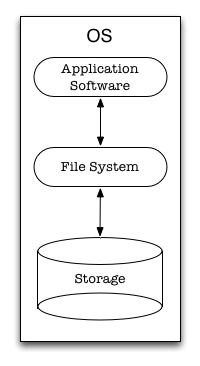
\includegraphics[scale=0.8]{pics/das.eps} \\
\end{center}
\verb+ssh lab 'df -hT /'+
\vfill

\subsection{Basic Disk Concepts: Storage Models}
Network Attached Storage (NAS)
\vfill
\begin{center}
	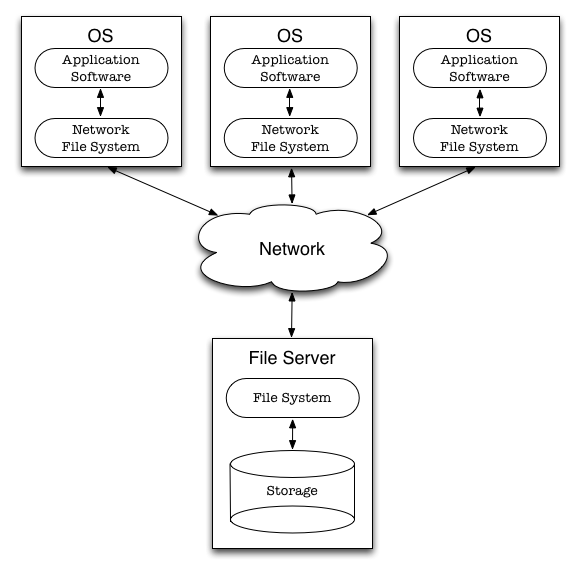
\includegraphics[scale=0.5]{pics/nas.eps} \\
\end{center}
\verb+ssh lab 'df -hT /home/$(whoami)'+
\vfill

\subsection{Basic Disk Concepts: Storage Models}
Storage Area Networks (SAN)
\vfill
\begin{center}
	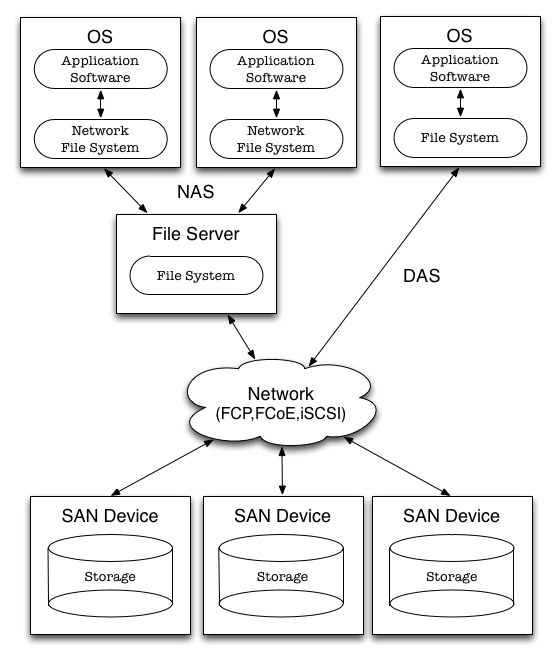
\includegraphics[scale=0.5]{pics/san-nas-das.eps} \\
\end{center}
\vfill

\subsection{Basic Disk Concepts: Storage Models}
Cloud Storage (Examples: EBS, S3)
\vfill
\begin{center}
	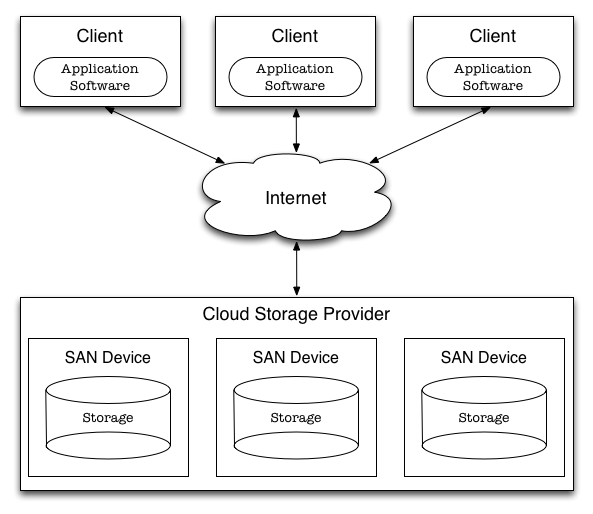
\includegraphics[scale=0.6]{pics/cloud-storage.eps} \\
\end{center}
\vfill

%\subsection{Basic Disk Concepts: Storage Models: Cloud Storage}
%\begin{verbatim}
%$ aws ec2 describe-instances
%[...]
%/dev/sda1	ebs	None	paravirtual
%BLOCKDEVICEMAPPINGS	/dev/sda
%EBS	2014-01-25T20:18:19.000Z	True	attached vol-a0d000d6
%[...]
%\end{verbatim}
%
%
%\subsection{Basic Disk Concepts: Storage Models: Cloud Storage}
%
%30 min. exercise: \\
%
%\begin{itemize}
%	\item create two instances
%	\item create a 1GB volume and attach it to one of the instances
%	\item create a new filesystem on the volume and mount it
%	\item create a file on the new filesystem
%	\item terminate the first instance
%	\item attach the volume to the second instance
%	\item retrieve the file from the volume via the second instance
%\end{itemize}
%
%If time permits, repeat using a Linux instance.
%\vspace{.25in}
%Useful commands: \\
%{\tt aws ec2 create-volume}, {\tt aws ec2 attach-volume}, {\tt
%format(1M)}, {\tt newfs(1M)}, {\tt mount(8)}
%
%\subsection{Basic Disk Concepts: Storage Models: Cloud Storage}
%\begin{verbatim}
%$ aws ec2 create-volume --size 1 --availability-zone us-east-1d
%[...]
%$ aws ec2 attach-volume --volume-id vol-9d3aeaeb --instance-id \
%        i-dd74f0f3 --device /dev/sdh
%[...]
%$ ssh <hostname>
%# format
%format> fdisk
%format> verify
%format> label
%# newfs /dev/rdsk/c1t2160d0s0
%[...]
%# mount /dev/dsk/c1t2160d0s0 /mnt
%# df -Th /mnt
%[...]
%# fstyp -v /dev/rdsk/c1t2160d0s0  | more
%[...]
%\end{verbatim}

\newpage
\vspace*{\fill}
\begin{center}
	\Hugesize
		Basic Disk Concepts \\ [1em]
	\hspace*{5mm}
	\blueline\\
	\hspace*{5mm}\\
		Disk Devices
\end{center}
\vspace*{\fill}


\subsection{Basic Disk Concepts: Disk Devices}
	\begin{center}
		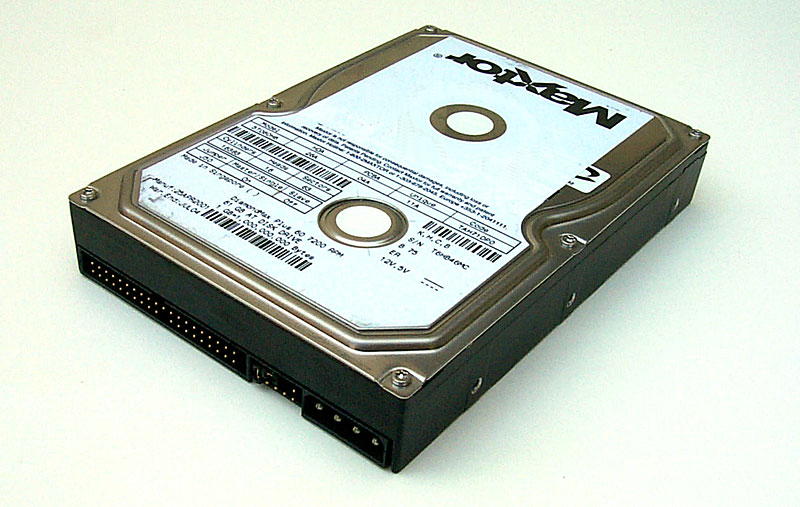
\includegraphics[scale=0.9]{pics/ide-drive.eps} \\
	\end{center}

\subsection{Basic Disk Concepts: Disk Devices}
Security affects everything. \\
\begin{center}
	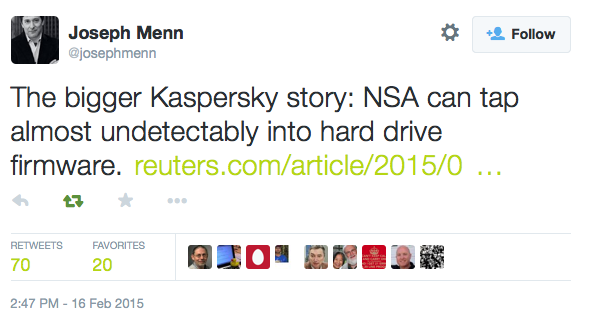
\includegraphics[scale=0.9]{pics/equation-tweet.eps} \\
	\verb+https://t.co/eM6XpATITQ+
\end{center}

\subsection{Basic Disk Concepts: Disk Devices}
	\begin{center}
		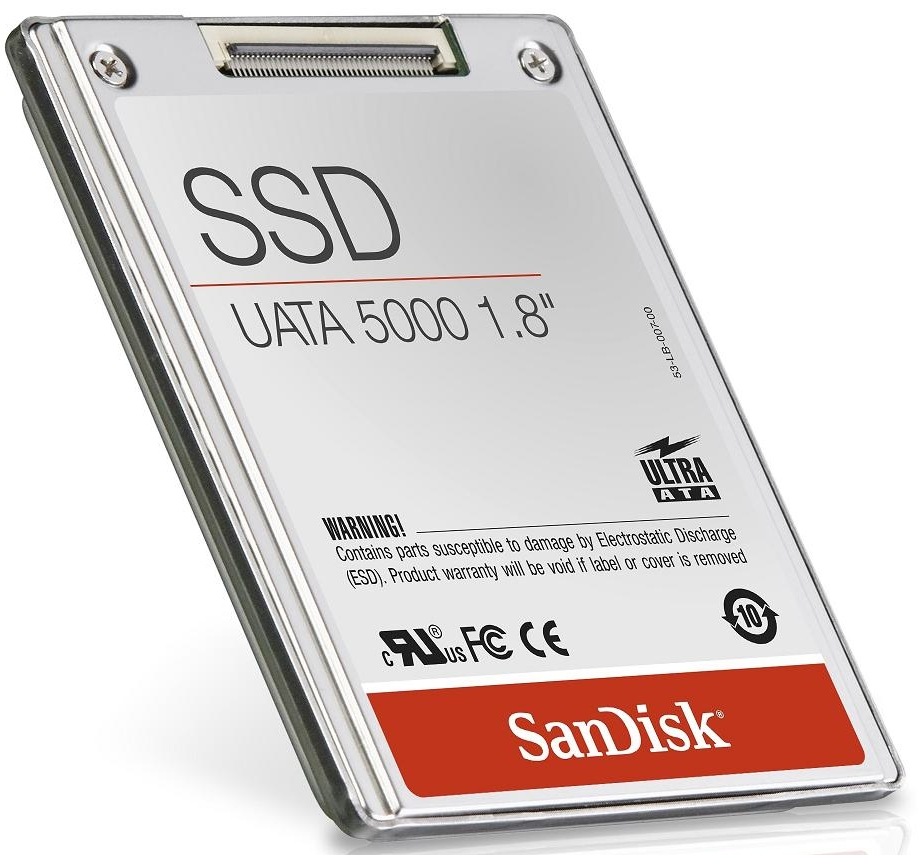
\includegraphics[scale=0.5]{pics/ssd.eps} \\
	\end{center}

\subsection{Basic Disk Concepts: Disk Devices}
	\begin{center}
		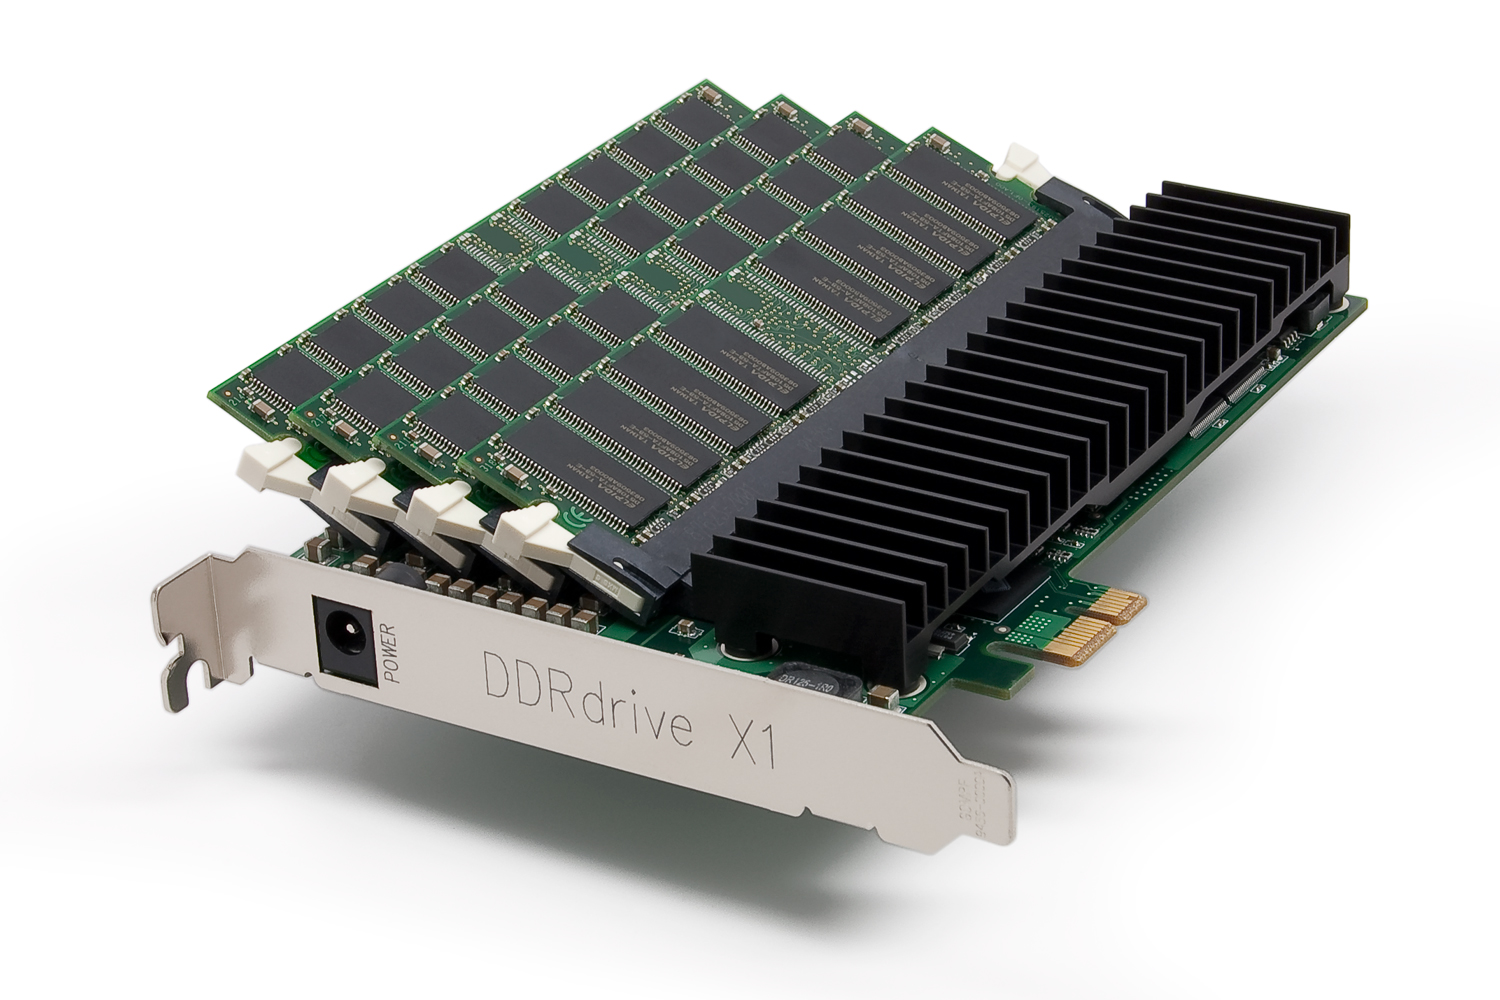
\includegraphics[scale=0.5]{pics/ddrdrive.eps} \\
	\end{center}

\subsection{Basic Disk Concepts: Disk Devices}
\begin{figure}[hb]
	\begin{center}
		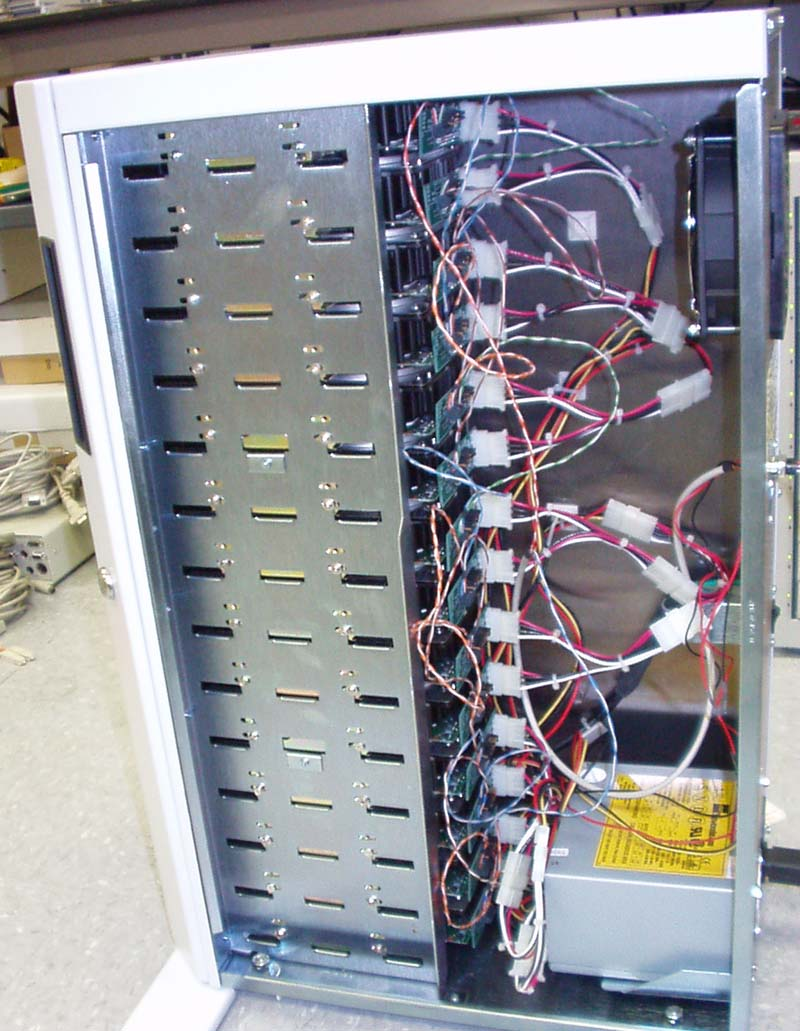
\includegraphics[scale=0.5]{pics/jbod-inside.eps}
		\hspace*{15mm}
		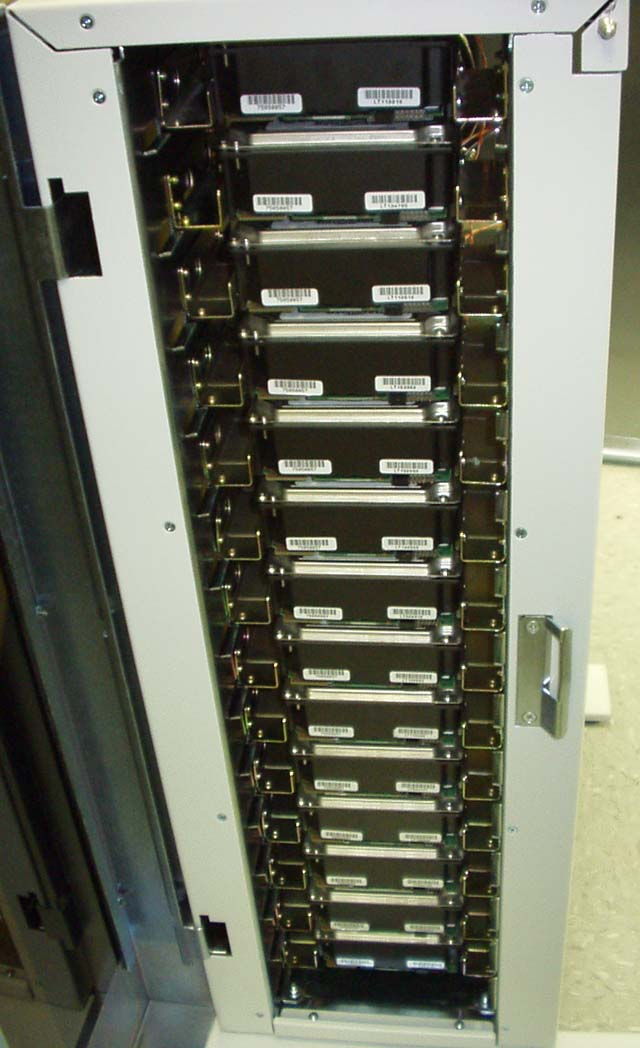
\includegraphics[scale=0.5]{pics/jbod-front.eps} \\
	\end{center}
\end{figure}


\subsection{Basic Disk Concepts: Disk Devices}
	\begin{center}
		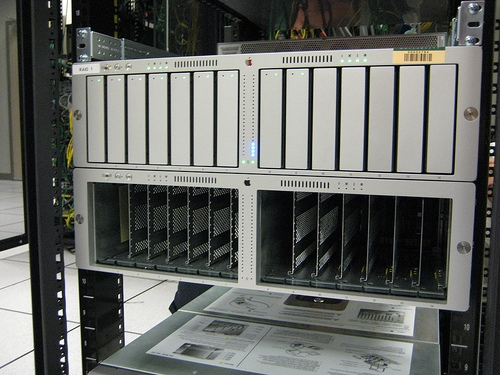
\includegraphics[scale=0.9]{pics/xraid.eps} \\
	\end{center}


\subsection{Basic Disk Concepts: Disk Devices}
	\begin{center}
		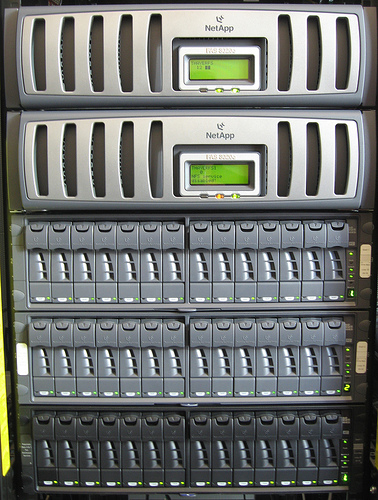
\includegraphics[scale=0.7]{pics/netapp.eps} \\
	\end{center}

\newpage
\vspace*{\fill}
\begin{center}
	\Hugesize
		Basic Disk Concepts \\ [1em]
	\hspace*{5mm}
	\blueline\\
	\hspace*{5mm}\\
		Disk Interfaces
\end{center}
\vspace*{\fill}

\subsection{Basic Disk Concepts: Disk Interfaces: SCSI}
\vfill
	\begin{center}
		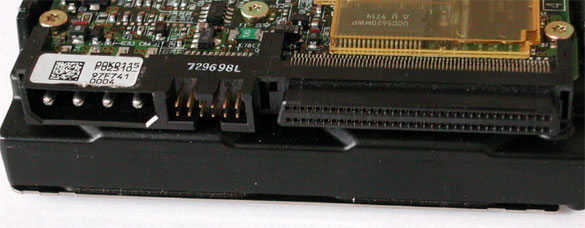
\includegraphics[scale=1.0]{pics/scsi-disk.eps} \\
	\end{center}
\vfill

% IDE
\subsection{Basic Disk Concepts: Disk Interfaces: ATA}
\vfill
	\begin{center}
		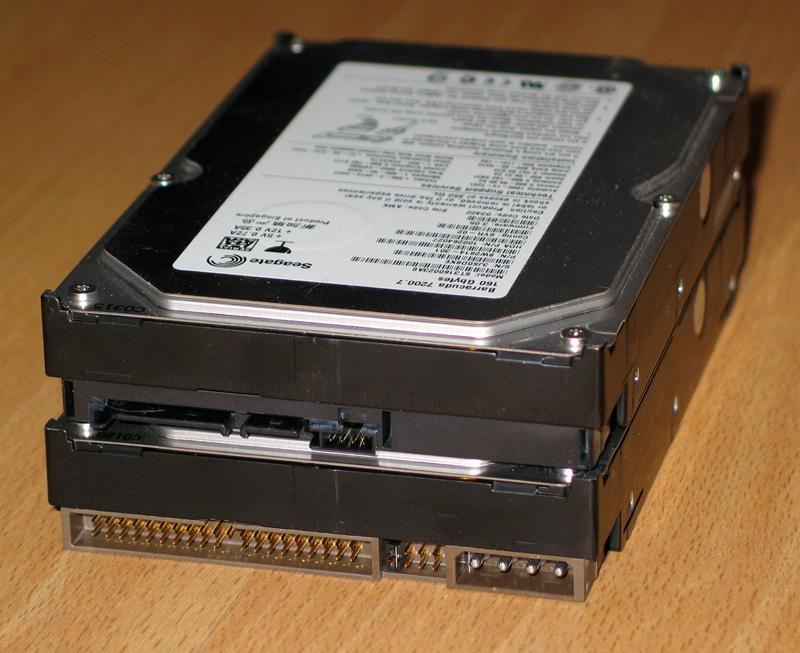
\includegraphics[scale=1.1]{pics/satavide.eps} \\
	\end{center}
\vfill

\subsection{Basic Disk Concepts: Disk Interfaces: ATA}
\vfill
	\begin{center}
		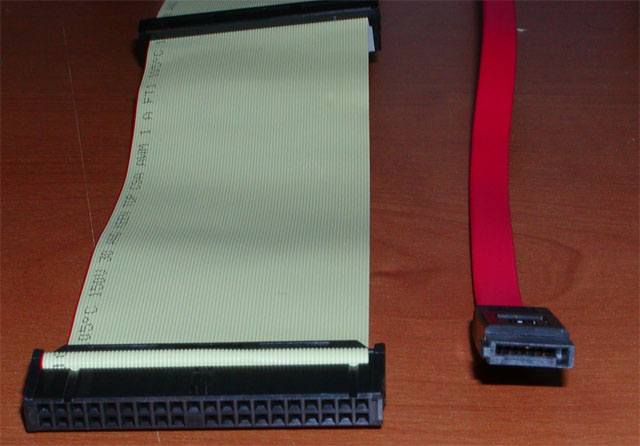
\includegraphics[scale=0.8]{pics/satavpata.eps} \\
	\end{center}
\vfill


% FC

\subsection{Basic Disk Concepts: Disk Interfaces: Fibre Channel}
\vfill
	\begin{center}
		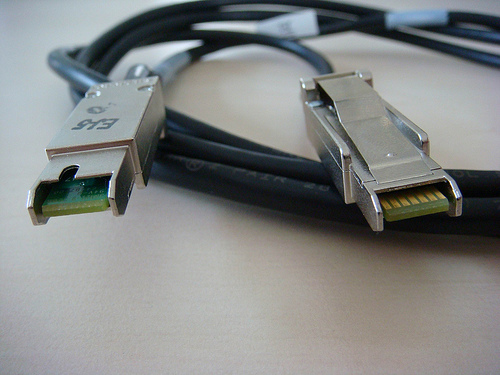
\includegraphics[scale=0.9]{pics/fc-connector.eps} \\
	\end{center}
\vfill

\subsection{Basic Disk Concepts: Disk Interfaces: Fibre Channel}
\vfill
	\begin{center}
		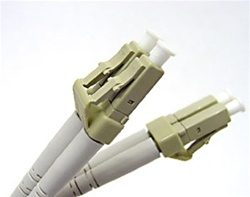
\includegraphics[scale=1.5]{pics/fc-optical.eps} \\
	\end{center}
\vfill

\subsection{Basic Disk Concepts: Disk Interfaces: Fibre Channel}
\vfill
	\begin{center}
		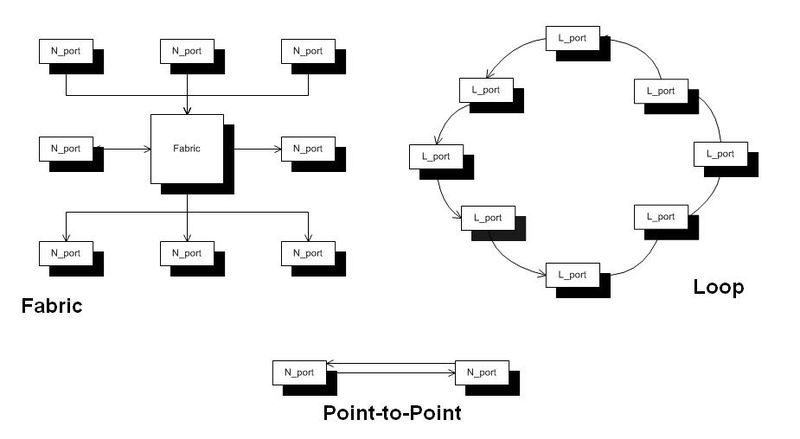
\includegraphics[scale=1.0]{pics/fc-topologies.eps} \\
	\end{center}
\vfill

\subsection{Basic Disk Concepts: Disk Interfaces: Fibre Channel}
\vfill
	\begin{center}
		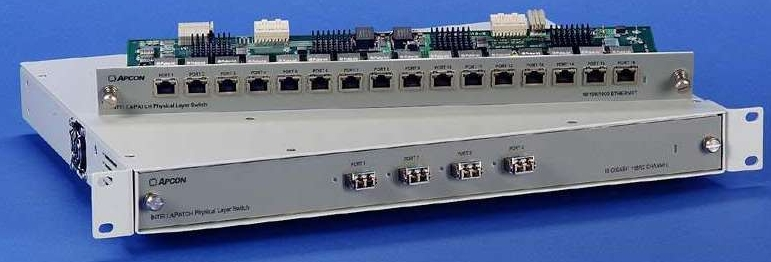
\includegraphics[scale=0.8]{pics/fc-switch.eps} \\
	\end{center}
\vfill

\subsection{Basic Disk Concepts: Disk Interfaces: Fibre Channel}
\vfill
	\begin{center}
		\includegraphics[scale=0.4]{pics/fc-switched.eps} \\
	\end{center}
\vfill

% SANs
\subsection{Basic Disk Concepts: Disk Interfaces: SANs}
\begin{itemize}
	\item ATA over Ethernet ({\em AoE}):
		\begin{itemize}
			\item create low-cost SAN
			\item ATA encapsulated into Ethernet frames
		\end{itemize}
	\item Fibre Channel over Ethernet ({\em FCoE}):
		\begin{itemize}
			\item consolidate IP and FC/SAN networks
			\item FC encapsulated into Ethernet frames
		\end{itemize}

	\item *oE:
		\begin{itemize}
			\item no TCP/IP overhead
			\item restricted to a single Layer 2 network
			\item no inherent security features
		\end{itemize}
	\item iSCSI
		\begin{itemize}
			\item SCSI encapsulated in TCP/IP packets
		\end{itemize}
\end{itemize}

\newpage
\vspace*{\fill}
\begin{center}
	\Hugesize
		Basic Disk Concepts\\ [1em]
	\hspace*{5mm}
	\blueline\\
	\hspace*{5mm}\\
		Physical Disk Structure
\end{center}
\vspace*{\fill}

\subsection{Basic Disk Concepts: Disk Devices}
\vfill
	\begin{center}
		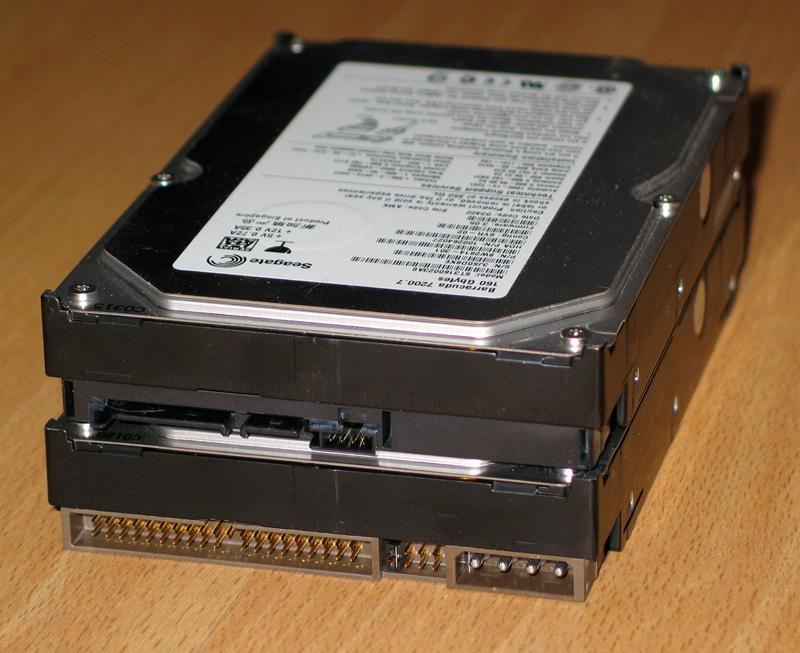
\includegraphics[scale=1.2]{pics/satavide.eps} \\
	\end{center}
\vfill


\subsection{Basic Disk Concepts: Disk Devices}
%\begin{figure}[hb]
	\begin{center}
		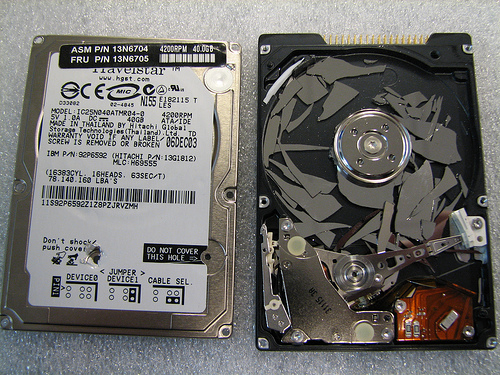
\includegraphics[scale=0.9]{pics/busted-disk.eps} \\
	\end{center}
%\end{figure}

\subsection{Basic Disk Concepts: Disk Devices}
\vfill
	\begin{center}
		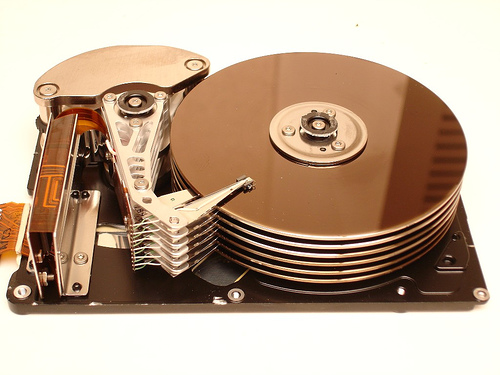
\includegraphics[scale=0.9]{pics/6platter.eps} \\
	\end{center}
\vfill

\subsection{Basic Disk Concepts: Physical Disk Structure}
\vfill
	\begin{center}
		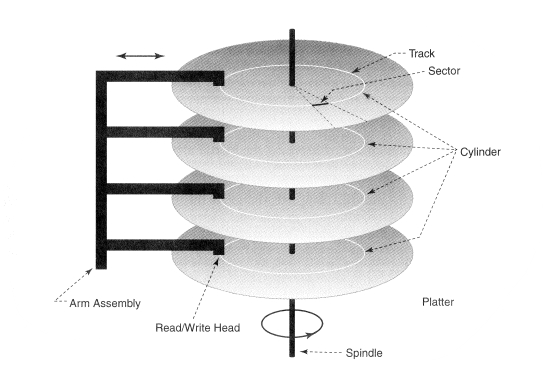
\includegraphics[scale=1.2]{pics/cylinders.eps} \\
	\end{center}
\vfill

\subsection{Basic Disk Concepts: Physical Disk Structure}
Hard drive performance determined by:
\begin{itemize}
	\item seek time
	\item rotational latency
	\item internal data rate
	\item a few other negligible factors (external data rate, command
		overhead, access time, etc.)
\end{itemize}

\subsection{Basic Disk Concepts: Disk Devices}
\begin{center}
	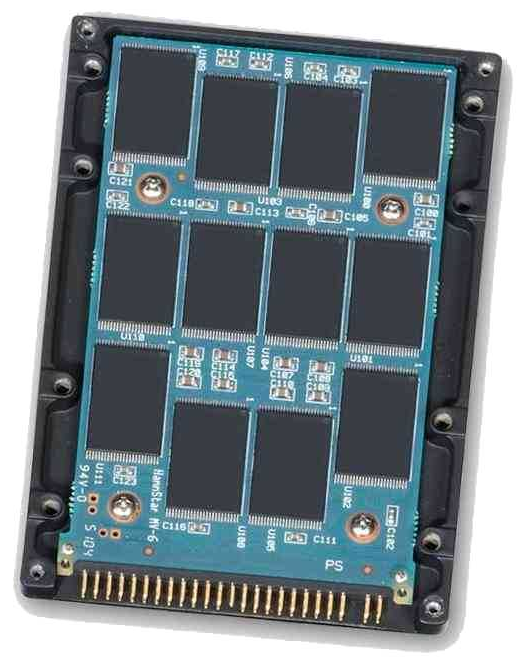
\includegraphics[scale=2]{pics/ssd-open.eps} \\
\end{center}


\newpage
\vspace*{\fill}
\begin{center}
	\Hugesize
		Basic Disk Concepts\\ [1em]
	\hspace*{5mm}
	\blueline\\
	\hspace*{5mm}\\
		Partitions
\end{center}
\vspace*{\fill}

\subsection{Basic Disk Concepts: Partitions}
	\begin{center}
		\includegraphics[scale=1.0]{pics/disk-structure.eps} \\
		\tiny Source: SGI Techpubs \\
	\end{center}

\subsection{Basic Disk Concepts: Partitions}
	\begin{center}
		\includegraphics[scale=0.7]{pics/disk.partition.eps}
	\end{center}


\subsection{Basic Disk Concepts: Partitions}
	\begin{center}
		\includegraphics[scale=0.9]{pics/partition.eps} \\
		\tiny Source: NetBSD Guide \\
	\end{center}

\subsection{Basic Disk Concepts: Partitions}
NetBSD example (from {\tt disklabel(8)})

\begin{tabular}{ l l c }
Partition 'a': & / & \\
Partition 'b': & swap & \\
Partition 'e': & /home & \\
\end{tabular}

\begin{verbatim}
#        size    offset   fstype [fsize bsize cpg/sgs]
a:  20972385        63   4.2BSD   4096 32768  1180  # (Cyl.      0*- 20805)
b:   1048320  20972448     swap                     # (Cyl.  20806 - 21845)
c:  78140097        63   unused      0     0        # (Cyl.      0*- 77519)
d:  78140160         0   unused      0     0        # (Cyl.      0 - 77519)
e:  56119392  22020768   4.2BSD   4096 32768 58528  # (Cyl.  21846 - 77519)
\end{verbatim}

\subsection{Basic Disk Concepts: Partitions}
NetBSD example (from {\tt disklabel(8)})

\begin{tabular}{ l l c }
Partition 'a': & / & 10 GB\\
Partition 'b': & swap & \\
Partition 'e': & /home & 26 GB\\
\end{tabular}

\begin{verbatim}
#        size    offset   fstype [fsize bsize cpg/sgs]
a:  20972385        63   4.2BSD   4096 32768  1180  # (Cyl.      0*- 20805)
b:   1048320  20972448     swap                     # (Cyl.  20806 - 21845)
c:  78140097        63   unused      0     0        # (Cyl.      0*- 77519)
d:  78140160         0   unused      0     0        # (Cyl.      0 - 77519)
e:  56119392  22020768   4.2BSD   4096 32768 58528  # (Cyl.  21846 - 77519)
\end{verbatim}


\subsection{Basic Disk Concepts: Partitions}
Solaris example (from {\tt format(1m)}):
\begin{verbatim}
Current partition table (original):
Total disk cylinders available: 38758 + 2 (reserved cylinders)

Part      Tag    Flag     Cylinders         Size            Blocks
  0       root    wm       3 -  3764        3.62GB    (3762/0/0)   7584192
  1       swap    wu    3765 -  4364      590.62MB    (600/0/0)    1209600
  2     backup    wm       0 - 38757       37.26GB    (38758/0/0) 78136128
  3 unassigned    wm       0                0         (0/0/0)            0
  4 unassigned    wm       0                0         (0/0/0)            0
  5 unassigned    wm       0                0         (0/0/0)            0
  6 unassigned    wm       0                0         (0/0/0)            0
  7       home    wm    4365 - 38757       33.06GB    (34393/0/0) 69336288
  8       boot    wu       0 -     0        0.98MB    (1/0/0)         2016
  9 alternates    wu       1 -     2        1.97MB    (2/0/0)         4032
\end{verbatim}

\subsection{Basic Disk Concepts: Partitions}
Linux example (from {\tt fdisk(8)}):
\begin{verbatim}
Disk /dev/sda: 80.0 GB, 80000000000 bytes
255 heads, 63 sectors/track, 9726 cylinders
Units = cylinders of 16065 * 512 = 8225280 bytes

   Device Boot      Start         End      Blocks   Id  System
/dev/sda1   *           1          33      265041   83  Linux
/dev/sda2              34        9726    77859022+  83  Linux
\end{verbatim}

\subsection{Basic Disk and Filesystem Concepts: RAID and Logical Volumes}
\begin{itemize}
	\item allow file systems to be larger than the physical size of a disk
	\item inrease I/O performance when {\em striped}
	\item fault tolerant when {\em mirrored} or {\em plexed}
\end{itemize}
\vfill
\begin{center}
        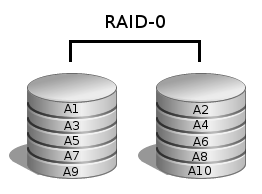
\includegraphics[scale=0.5]{pics/raid-0.eps}
        \hspace{.5in}
        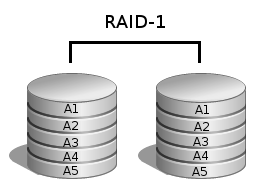
\includegraphics[scale=0.5]{pics/raid-1.eps} \\
        \vspace{.2in}
        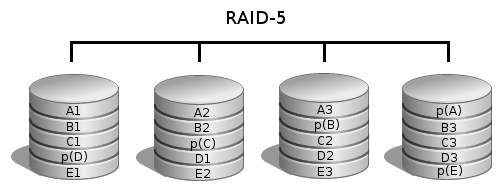
\includegraphics[scale=0.5]{pics/raid-5.eps}
\end{center}
\vfill


\newpage
\vspace*{\fill}
\begin{center}
    \Hugesize
        Hooray! \\ [1em]
    \hspace*{5mm}
    \blueline\\
    \hspace*{5mm}\\
        5 Minute Break
\end{center}
\vspace*{\fill}

\newpage
\vspace*{\fill}
\begin{center}
	\Hugesize
		Basic Filesystem Concepts\\ [1em]
	\hspace*{5mm}
	\blueline\\
	\hspace*{5mm}\\
		Filesystem Layout
\end{center}
\vspace*{\fill}

\subsection{Basic Filesystem Concepts}
All partitions -- with the exception of the {\em root} (or \verb+/+) partition
-- can be {\em mounted} anywhere in the filesystem hierarchy.
\\

\begin{center}
	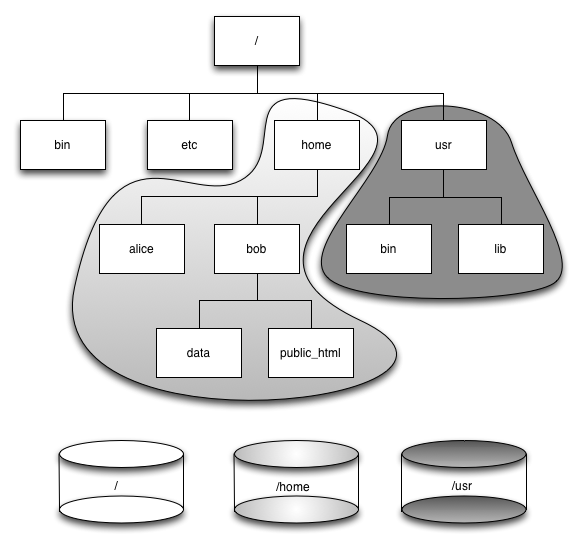
\includegraphics[scale=0.5]{pics/filesystem-tree-mountpoints.eps} \\
\end{center}

%\subsection{Basic Filesystem Concepts}
%All partitions -- with the exception of the {\em root} (or \verb+/+) partition
%-- can be {\em mounted} anywhere in the filesystem hierarchy.
%\\
%
%\begin{center}
%\includegraphics[scale=0.7]{pics/fs-tree-disks.eps} \\
%\end{center}
%
\subsection{Basic Filesystem Concepts}
All partitions -- with the exception of the {\em root} (or \verb+/+) partition
-- can be {\em mounted} anywhere in the filesystem hierarchy.
\\

The file \verb+/etc/fstab+ (see fstab(5)) specifies which disks / partitions
to mount where:
\\
\begin{verbatim}
/dev/wd0a   /        ffs    rw 1 1
/dev/cgd1a  none     swap   sw 0 0
/dev/cgd0a  /home    ffs    rw 1 2
/ignoreme   /tmp     mfs    rw,-b4096,-f512,-s262144 0 0
kernfs      /kern    kernfs rw
procfs      /proc    procfs rw,noauto
ptyfs       /dev/pts ptyfs  rw 0 0
\end{verbatim}
\Normalsize

\subsection{Basic Filesystem Concepts}
All partitions -- with the exception of the {\em root} (or \verb+/+) partition
-- can be {\em mounted} anywhere in the filesystem hierarchy.
\\

The file \verb+/etc/fstab+ (see fstab(5)) specifies which disks / partitions
to mount where:
\\
\small
\begin{verbatim}
# /etc/fstab: static file system information.
#
# Use 'vol_id --uuid' to print the universally unique identifier for a
# device; this may be used with UUID= as a more robust way to name devices
# that works even if disks are added and removed. See fstab(5).
#
# <file system> <mount point>   <type>  <options>       <dump>  <pass>
proc            /proc           proc    defaults        0       0
# / was on /dev/sda2 during installation
LABEL=ROOT      /       ext3    errors=remount-ro,acl   0       1
# /boot was on /dev/sda1 during installation
LABEL=BOOT      /boot   ext3    defaults,acl            0       2
# swap was on /dev/sda5 during installation
UUID=9329ae83-289d-4c3d-8756-f707c4bbb312 none            swap    sw
0       0
/dev/scd0       /media/cdrom0   udf,iso9660 user,noauto,exec,utf8 0       0
deathstar.phy.stevens-tech.edu:/export/nfs-sw/opt    /opt            nfs ro,rsize=32768,intr,nolock  0 0
deathstar.phy.stevens-tech.edu:/export/srcit-dist    /mnt/srcit-dist  nfs ro,rsize=32768,intr,nolock  0 0
corsario.cs.stevens-tech.edu:/export/people          /mnt/legacy/people nfs rw,rsize=32768,wsize=32768,intr,lock   0 0
corsario.cs.stevens-tech.edu:/export/faculty         /mnt/legacy/faculty nfs rw,rsize=32768,wsize=32768,intr,lock  0 0

\end{verbatim}
\Normalsize


\subsection{Basic Filesystem Concepts}
All partitions -- with the exception of the {\em root} (or \verb+/+) partition
-- can be {\em mounted} anywhere in the filesystem hierarchy.
\\

To see what filesystems are currently mounted, run \verb+mount(8)+:
\\

\begin{verbatim}
/dev/wd0a on / type ffs (local)
/dev/cgd0a on /home type ffs (local)
mfs:276 on /tmp type mfs (synchronous, local)
kernfs on /kern type kernfs (local)
ptyfs on /dev/pts type ptyfs (local)
\end{verbatim}


\subsection{Basic Filesystem Concepts}
\\

\small
\begin{verbatim}
$ mount
/dev/sda2 on / type ext3 (rw,errors=remount-ro,acl)
tmpfs on /lib/init/rw type tmpfs (rw,nosuid,mode=0755)
proc on /proc type proc (rw,noexec,nosuid,nodev)
sysfs on /sys type sysfs (rw,noexec,nosuid,nodev)
varrun on /var/run type tmpfs (rw,nosuid,mode=0755)
varlock on /var/lock type tmpfs (rw,noexec,nosuid,nodev,mode=1777)
udev on /dev type tmpfs (rw,mode=0755)
tmpfs on /dev/shm type tmpfs (rw,nosuid,nodev)
devpts on /dev/pts type devpts (rw,noexec,nosuid,gid=5,mode=620)
fusectl on /sys/fs/fuse/connections type fusectl (rw)
lrm on /lib/modules/2.6.28-17-generic/volatile type tmpfs (rw,mode=755)
/dev/sda1 on /boot type ext3 (rw,acl)
securityfs on /sys/kernel/security type securityfs (rw)
automount(pid2623) on /home type autofs (rw,fd=4,pgrp=2623,minproto=2,maxproto=4)
deathstar.phy.stevens-tech.edu:/export/nfs-sw/opt on /opt type nfs (ro,rsize=32768,intr,nolock,addr=155.246.89.4)
deathstar.phy.stevens-tech.edu:/export/srcit-dist on /mnt/srcit-dist type nfs (ro,rsize=32768,intr,nolock,addr=155.246.89.4)
corsario.cs.stevens-tech.edu:/export/people on /mnt/legacy/people type nfs (rw,rsize=32768,wsize=32768,intr,lock,addr=155.246.89.20)
corsario.cs.stevens-tech.edu:/export/faculty on /mnt/legacy/faculty type nfs (rw,rsize=32768,wsize=32768,intr,lock,addr=155.246.89.20)
binfmt_misc on /proc/sys/fs/binfmt_misc type binfmt_misc (rw,noexec,nosuid,nodev)
deathstar.phy.stevens-tech.edu:/export/home/kamberov on /home/kamberov type nfs (rw,sync,intr,vers=3,sloppy,addr=155.246.89.4)
deathstar.phy.stevens-tech.edu:/export/home/mweiss on /home/mweiss type nfs (rw,sync,intr,vers=3,sloppy,addr=155.246.89.4)
deathstar.phy.stevens-tech.edu:/export/home/jschauma on /home/jschauma type nfs (rw,sync,intr,vers=3,sloppy,addr=155.246.89.4)
\end{verbatim}
\Normalsize

\subsection{Basic Filesystem Concepts}
Some of the different kinds of filesystems:

\subsection{Basic Filesystem Concepts}
Some of the different kinds of filesystems:
\begin{itemize}
	\item ``Regular'' File Systems
	\item Journaling File Systems
	\item Network File Systems
	\item Various
\end{itemize}

\newpage
\vspace*{\fill}
\begin{center}
	\Hugesize
		Basic Filesystem Concepts\\ [1em]
	\hspace*{5mm}
	\blueline\\
	\hspace*{5mm}\\
		The UNIX Filesystem
\end{center}
\vspace*{\fill}

\subsection{Basic Filesystem Concepts: The UNIX Filesystem}
The filesystem is responsible for storing the data on the disk.
So to read/write data, it needs to know in which physical blocks the actual
data is located; ie how to map files to the disk blocks.

\subsection{Let's pretend we're a filesystem...}

\begin{verbatim}
aws ec2 create-volume --size 1 --availability-zone us-east-1a

aws ec2 attach-volume --volume-id  XXX --instance-id XXX --device /dev/sda2

dmesg

echo hello | dd of=/dev/xbd2

dd if=/dev/xbd2 count=6 | hexdump -C

echo hello | dd of=/dev/xbd2 seek=1024

dd if=/dev/xbd2 count=2048 2>/dev/null | hexdump -C

printf "\x7\x4\x4hello" | dd of=/dev/xbd2
\end{verbatim}




\subsection{Basic Filesystem Concepts: The UNIX Filesystem}
\vspace*{\fill}
\begin{center}
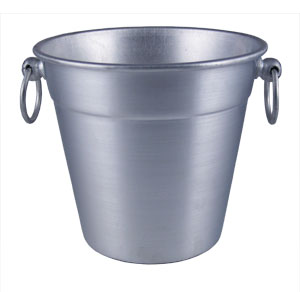
\includegraphics[scale=0.95]{pics/bucket.eps} \\
\end{center}
\vspace*{\fill}

\subsection{Basic Filesystem Concepts: The UNIX Filesystem}
\begin{center}
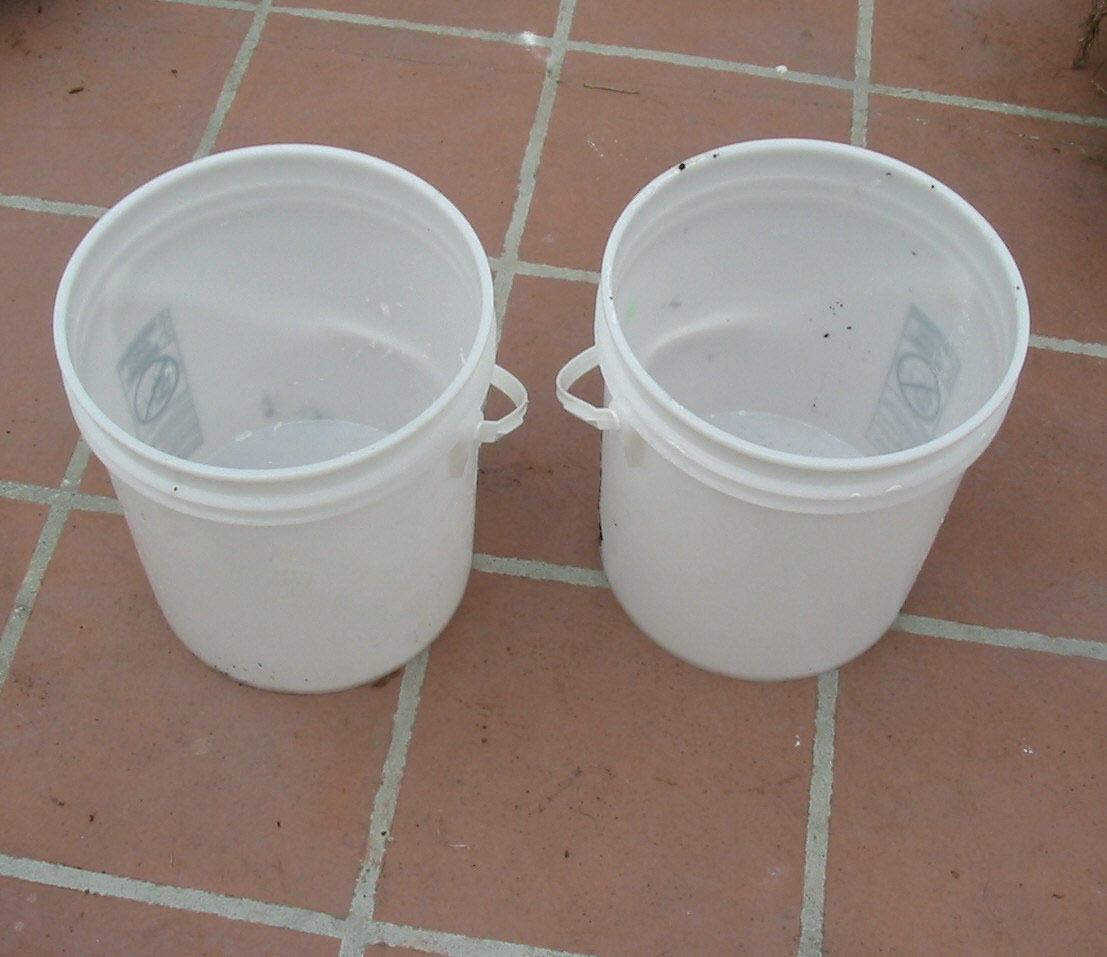
\includegraphics[scale=0.95]{pics/two-buckets.eps} \\
\end{center}

\subsection{Basic Filesystem Concepts: The UNIX Filesystem}
\vspace*{\fill}
\begin{center}
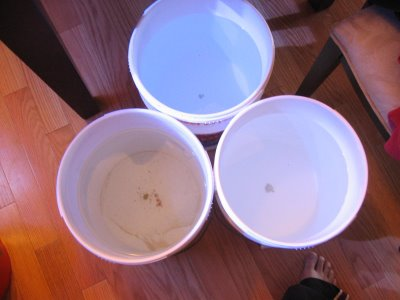
\includegraphics[scale=1.0]{pics/three-buckets.eps} \\
\end{center}
\vspace*{\fill}

\subsection{Basic Filesystem Concepts: The UNIX Filesystem}
\vspace*{\fill}
\begin{center}
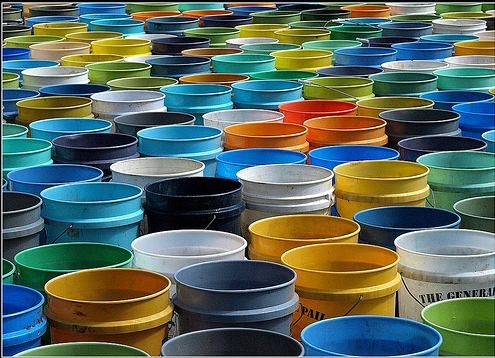
\includegraphics[scale=0.95]{pics/buckets.eps} \\
\end{center}
\vspace*{\fill}

\subsection{Basic Filesystem Concepts: The UNIX Filesystem}
\vspace*{\fill}
\begin{center}
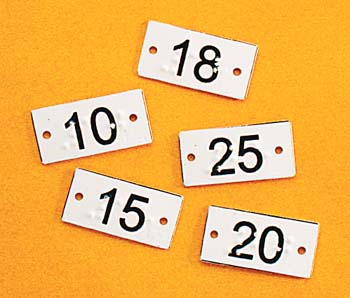
\includegraphics[scale=0.95]{pics/labels.eps} \\
\end{center}
\vspace*{\fill}

\subsection{Basic Filesystem Concepts: The UNIX Filesystem}
\begin{center}
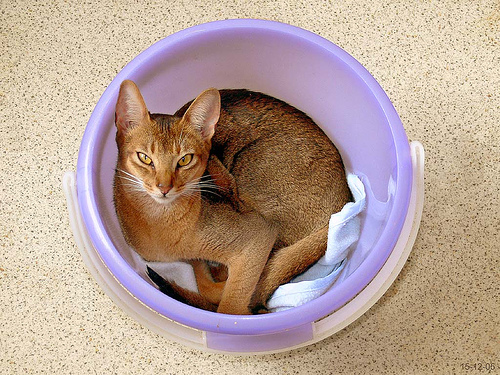
\includegraphics[scale=0.95]{pics/one-bucket-full.eps} \\
\end{center}

\subsection{Basic Filesystem Concepts: The UNIX Filesystem}
\vspace*{\fill}
\begin{center}
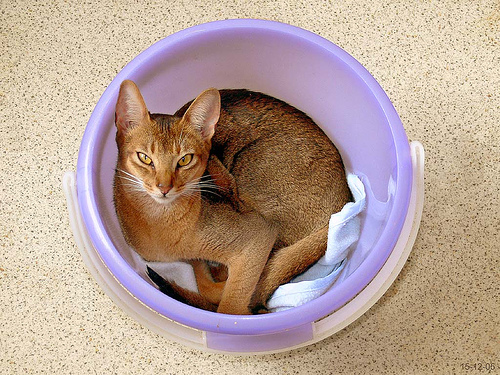
\includegraphics[scale=0.5]{pics/one-bucket-full.eps}
\hspace*{5mm}
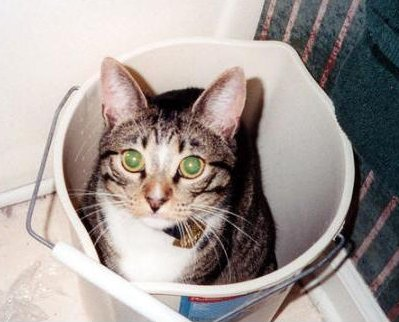
\includegraphics[scale=0.6]{pics/cat-in-bucket.eps}
\end{center}
\vspace*{\fill}

\subsection{Basic Filesystem Concepts: The UNIX Filesystem}
\vspace*{\fill}
\begin{center}
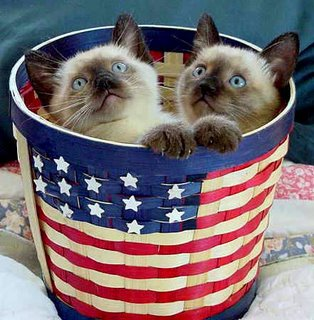
\includegraphics[scale=0.95]{pics/two-cats-one-bucket.eps} \\
\end{center}
\vspace*{\fill}

\subsection{Basic Filesystem Concepts: The UNIX Filesystem}
\begin{center}
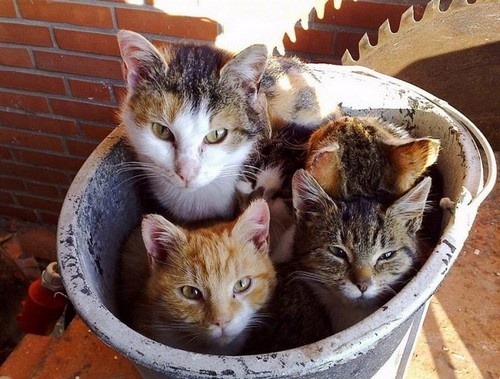
\includegraphics[scale=0.9]{pics/several-cats.eps} \\
\end{center}

\subsection{Basic Filesystem Concepts: The UNIX Filesystem}
\vspace*{\fill}
\begin{center}
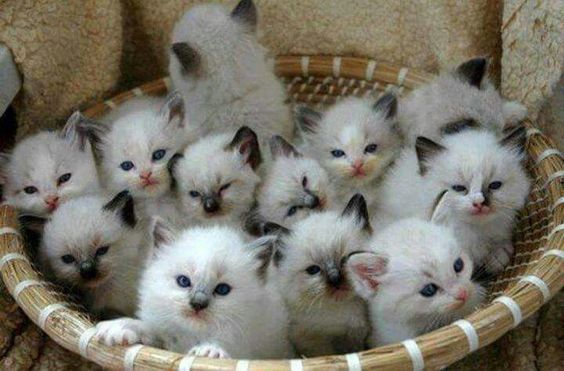
\includegraphics[scale=0.9]{pics/many-cats-in-basket.eps} \\
\end{center}
\vspace*{\fill}

\subsection{Basic Filesystem Concepts: The UNIX Filesystem}
\vspace*{\fill}
\begin{center}
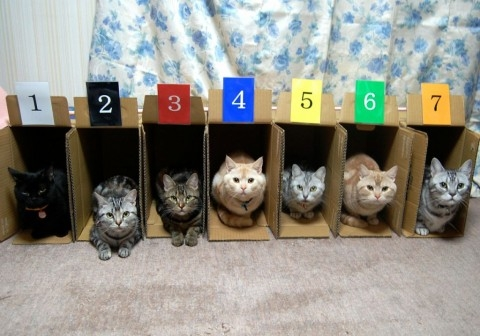
\includegraphics[scale=1.0]{pics/numbered-cats.eps} \\
\end{center}
\vspace*{\fill}

\subsection{Basic Filesystem Concepts: The UNIX Filesystem}
The filesystem is responsible for storing the data on the disk.
So to read/write data, it needs to know in which physical blocks the actual
data is located; ie how to map files to the disk blocks.
\\

Components of the Berkeley Fast Filesystem:
\\

\newcolumntype{S}{>{\centering\arraybackslash} m{.4\linewidth} }
\begin{tabular}{ p{10cm} S }
\begin{itemize}
	\item set of {\em inode} storage cells
\end{itemize}
{\tt df -i}
& \multirow{2}{*}{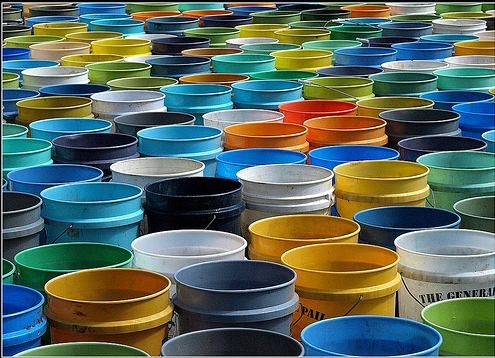
\includegraphics[scale=0.5]{pics/buckets.eps}} \\
\end{tabular}

\subsection{Basic Filesystem Concepts: The UNIX Filesystem}
The filesystem is responsible for storing the data on the disk.
So to read/write data, it needs to know in which physical blocks the actual
data is located; ie how to map files to the disk blocks.
\\

Components of the Berkeley Fast Filesystem:
\\

\begin{tabular}{ p{10cm} S }
\begin{itemize}
	\item set of {\em inode} storage cells
	\item set of scattered ``superblocks''
\end{itemize}
{\tt newfs -N /dev/rdsk/c1t2160d0s0}
& \multirow{2}{*}{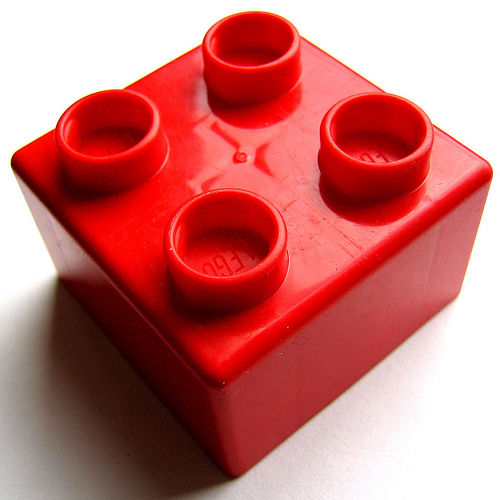
\includegraphics[scale=0.3]{pics/lego.eps}} \\
\end{tabular}

\subsection{Basic Filesystem Concepts: The UNIX Filesystem}
The filesystem is responsible for storing the data on the disk.
So to read/write data, it needs to know in which physical blocks the actual
data is located; ie how to map files to the disk blocks.
\\

Components of the Berkeley Fast Filesystem:
\\

\begin{tabular}{ p{10cm} S }
\begin{itemize}
	\item set of {\em inode} storage cells
	\item set of scattered ``superblocks''
	\item map of disk blocks
\end{itemize}
& \multirow{2}{*}{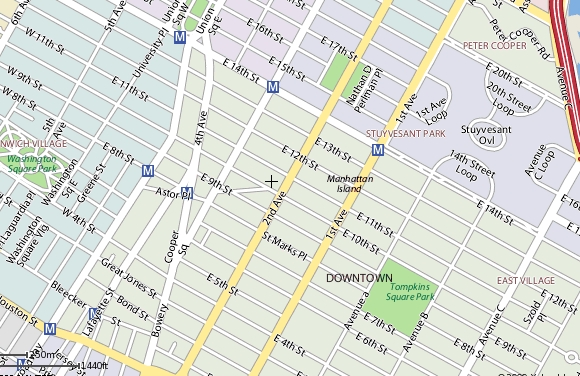
\includegraphics[scale=0.5]{pics/map.eps}} \\
\end{tabular}

\subsection{Basic Filesystem Concepts: The UNIX Filesystem}
The filesystem is responsible for storing the data on the disk.
So to read/write data, it needs to know in which physical blocks the actual
data is located; ie how to map files to the disk blocks.
\\

Components of the Berkeley Fast Filesystem:
\\

\begin{tabular}{ p{10cm} S }
\begin{itemize}
	\item set of {\em inode} storage cells
	\item set of scattered ``superblocks''
	\item map of disk blocks
	\item block usage summary
\end{itemize}
{\tt fstyp -v /dev/rdsk/c1t2160d0s0  | more}
& \multirow{2}{*}{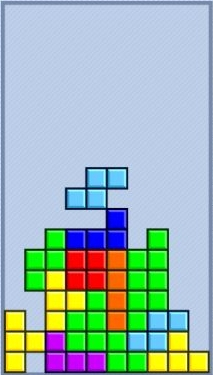
\includegraphics[scale=0.5]{pics/tetris.eps}} \\
\end{tabular}

\subsection{Basic Filesystem Concepts: The UNIX Filesystem}
The filesystem is responsible for storing the data on the disk.
So to read/write data, it needs to know in which physical blocks the actual
data is located; ie how to map files to the disk blocks.
\\

Components of the Berkeley Fast Filesystem:
\\

\begin{tabular}{ p{10cm} S }
\begin{itemize}
	\item set of {\em inode} storage cells
	\item set of scattered ``superblocks''
	\item map of disk blocks
	\item block usage summary
	\item set of data blocks
\end{itemize}
& \multirow{2}{*}{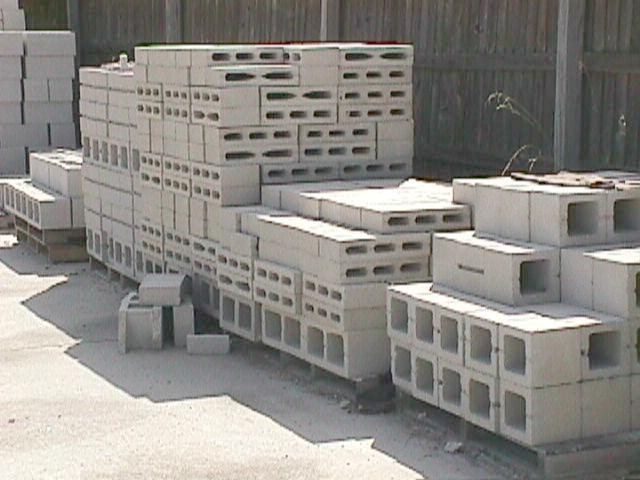
\includegraphics[scale=0.3]{pics/block.eps}} \\
\end{tabular}

\subsection{Basic Filesystem Concepts: The UNIX Filesystem}
\begin{center}
	\includegraphics[scale=0.8]{pics/ufs-details.eps} \\
\end{center}
\vspace*{\fill}

\subsection{Basic Filesystem Concepts: The UNIX Filesystem}
Information stored in an {\em inode}:

\subsection{Basic Filesystem Concepts: The UNIX Filesystem}
Information stored in an {\em inode}:
\begin{itemize}
	\item user owner and group owner ID's
\end{itemize}

\subsection{Basic Filesystem Concepts: The UNIX Filesystem}
Information stored in an {\em inode}:
\begin{itemize}
	\item user owner and group owner ID's
	\item file type
\end{itemize}

\subsection{Basic Filesystem Concepts: The UNIX Filesystem}
Information stored in an {\em inode}:
\begin{itemize}
	\item user owner and group owner ID's
	\item file type
	\item access mode (permissions)
\end{itemize}

\subsection{Basic Filesystem Concepts: The UNIX Filesystem}
Information stored in an {\em inode}:
\begin{itemize}
	\item user owner and group owner ID's
	\item file type
	\item access mode (permissions)
	\item file access and modification time
\end{itemize}

\subsection{Basic Filesystem Concepts: The UNIX Filesystem}
Information stored in an {\em inode}:
\begin{itemize}
	\item user owner and group owner ID's
	\item file type
	\item access mode (permissions)
	\item file access and modification time
	\item file status modification time
\end{itemize}

\subsection{Basic Filesystem Concepts: The UNIX Filesystem}
Information stored in an {\em inode}:
\begin{itemize}
	\item user owner and group owner ID's
	\item file type
	\item access mode (permissions)
	\item file access and modification time
	\item file status modification time
	\item number of links to the file
\end{itemize}

\subsection{Basic Filesystem Concepts: The UNIX Filesystem}
Information stored in an {\em inode}:
\begin{itemize}
	\item user owner and group owner ID's
	\item file type
	\item access mode (permissions)
	\item file access and modification time
	\item file status modification time
	\item number of links to the file
	\item size of the file
\end{itemize}

\subsection{Basic Filesystem Concepts: The UNIX Filesystem}
Information stored in an {\em inode}:
\begin{itemize}
	\item user owner and group owner ID's
	\item file type
	\item access mode (permissions)
	\item file access and modification time
	\item file status modification time
	\item number of links to the file
	\item size of the file
	\item disk device containing this file
\end{itemize}

\subsection{Basic Filesystem Concepts: The UNIX Filesystem}
Information stored in an {\em inode}:
\begin{itemize}
	\item user owner and group owner ID's
	\item file type
	\item access mode (permissions)
	\item file access and modification time
	\item file status modification time
	\item number of links to the file
	\item size of the file
	\item disk device containing this file
\end{itemize}

\begin{verbatim}
$ stat /etc/passwd
\end{verbatim}

\subsection{Basic Filesystem Concepts: The UNIX Filesystem}
File types:
\\

\begin{tabular}{ p{10cm} S }
\begin{itemize}
	\item regular files
\end{itemize}
& \multirow{2}{*}{\includegraphics[scale=0.7]{pics/file.eps}} \\
\end{tabular}
\\

\verb+$ stat /etc/passwd+


\subsection{Basic Filesystem Concepts: The UNIX Filesystem}
File types:
\\

\begin{tabular}{ p{10cm} S }
\begin{itemize}
	\item regular files
	\item directories
\end{itemize}
& \multirow{2}{*}{\includegraphics[scale=1.5]{pics/directory.eps}} \\
\end{tabular}
\\

\verb+$ stat /+

\subsection{Basic Filesystem Concepts: The UNIX Filesystem}
File types:
\\

\begin{tabular}{ p{10cm} S }
\begin{itemize}
	\item regular files
	\item directories
	\item special files
\end{itemize}
& \multirow{2}{*}{\includegraphics[scale=1.0]{pics/devices.eps}} \\
\end{tabular}
\\

\verb+$ file /dev/* | more+

\subsection{Basic Filesystem Concepts: The UNIX Filesystem}
File types:
\\

\begin{tabular}{ p{10cm} S }
\begin{itemize}
	\item regular files
	\item directories
	\item special files
	\item links
\end{itemize}
& \multirow{2}{*}{\includegraphics[scale=0.6]{pics/link.eps}} \\
\end{tabular}
\\

\begin{verbatim}
$ touch /tmp/foo
$ ln /tmp/foo /tmp/bar
$ stat /tmp/foo /tmp/bar
$ ln -sf /tmp/foo /tmp/bar
$ stat /tmp/foo /tmp/bar
\end{verbatim}

\subsection{Basic Filesystem Concepts: The UNIX Filesystem}
File types:
\\

\begin{tabular}{ p{10cm} S }
\begin{itemize}
	\item regular files
	\item directories
	\item special files
	\item links
	\item sockets
\end{itemize}
& \multirow{2}{*}{\includegraphics[scale=0.8]{pics/socket.eps}} \\
\end{tabular}
\\

\verb+$ stat /dev/log+

\subsection{Basic Filesystem Concepts: The UNIX Filesystem}
File types:
\\

\begin{tabular}{ p{10cm} S }
\begin{itemize}
	\item regular files
	\item directories
	\item special files
	\item links
	\item sockets
	\item named pipes
\end{itemize}
& \multirow{2}{*}{\includegraphics[scale=1.0]{pics/pipe.eps}} \\
\end{tabular}
\\

\begin{verbatim}
$ mkfifo /tmp/fifo
$ cat /tmp/fifo > /tmp/out &
$ stat /tmp/fifo | tee /tmp/fifo
$ cat /tmp/out
\end{verbatim}

\subsection{Homework}
Repeat the examples from class.  Make sure you understand the commands and
how they relate to the concepts we discussed.  Repeat for a different OS,
for example: \\

\begin{itemize}
	\item {\tt ami-3b361952} -- Fedora 23
	\item {\tt ami-f709a29c} -- FreeBSD 10.2
	\item {\tt ami-569ed93c} -- NetBSD 7.0
	\item {\tt ami-50ecc847} -- OmniOS 5.11
\end{itemize}

\vspace{.5in}
Remember to {\em shut down} your EC2 instances and to {\em delete} any unused ESB
volumes!

\vspace{.5in}
{\tt https://www.cs.stevens.edu/\~{}jschauma/615/s18-hw2.html}


\subsection{Reading}
\begin{itemize}
	\item \verb+https://is.gd/5mndwA+
	\item \verb+https://is.gd/ig4QP5+
	\item \verb+https://is.gd/9YeIKh+
\end{itemize}

\subsection{Reading}
Disk Interfaces:
\begin{itemize}
	\item SCSI:
		\begin{itemize}
			\item \verb+https://en.wikipedia.org/wiki/Scsi+
			\item scsi(4), scsictl(8);
		\end{itemize}
	\item ATA:
		\begin{itemize}
			\item \verb+http://www.ata-atapi.com/+
			\item \verb+https://en.wikipedia.org/wiki/Advanced_Technology_Attachment+
			\item \verb+https://en.wikipedia.org/wiki/Sata+
		\end{itemize}
\end{itemize}

\subsection{Reading}
Disk Interfaces:
\begin{itemize}
	\item Serial attached SCSI:
		\begin{itemize}
			\item \verb+https://en.wikipedia.org/wiki/Serial_attached_SCSI+
		\end{itemize}
	\item Fibre Channel:
		\begin{itemize}
			\item \verb+https://hsi.web.cern.ch/HSI/fcs/fcs.html+
			\item \verb+https://en.wikipedia.org/wiki/Fibrechannel+
		\end{itemize}
	\item AoE, FCoE, iSCSI:
		\begin{itemize}
			\item \verb+https://en.wikipedia.org/wiki/ATA_over_Ethernet+
			\item \verb+https://en.wikipedia.org/wiki/FCoE+
			\item \verb+https://en.wikipedia.org/wiki/ISCSI+
		\end{itemize}
\end{itemize}

\subsection{Reading}
Basic Disk Concepts:
\begin{itemize}
	\item disklabel(8), fdisk(8)
	\item format(1m)
\end{itemize}
RAID:
\begin{itemize}
	\item \verb+https://en.wikipedia.org/wiki/RAID+
\end{itemize}
Basic Filesystem Concepts:
\begin{itemize}
	\item \verb+https://is.gd/8KHnQj+
	\item \verb+https://is.gd/wGgJ0e+
	\item newfs(8)
\end{itemize}
NFS: \verb+https://is.gd/70yqMZ+

\end{document}
